\chapter{Réseaux sans fils sous Linux}
\section{Gestion du réseau sous Linux}

Une importante partie du projet consiste à pouvoir communiquer avec les interfaces sans fils dont disposent les appareils. En effet,
il est nécessaire d'une part, de récupérer des informations à propos de ces dernières et d'autre part, de les configurer pour
arriver à les utiliser de la manèére que nous le souhaitons. Pour gérer les interfaces sans fils, il est important de bien
distinguer deux niveaux : Les cartes réseaux\footnote{généralement abrégées \textbf{wiphy}, pour WIreless PHYsical device} , 
qui existent physiquement, et les interfaces qui pourraient être qualifiées de ``logiques'', qui utilisent ces cartes réseaux et 
sont utilisées pour envoyer et recevoir des données. Un type (Point d'acces, client, noeud mesh, monitor, ...) est associé à chaque 
interface, determinant son mode de fonctionnement. Une seule carte réseau peut être utilisée par plusieurs interfaces.

Historiquement, sous linux, la communication avec les interfaces se faisait avec des appels systémes ioctl\footnote{Abréviation
de Input Output ConTroL, il s'agit d'une fonction permettant de manipuler des fichiers spéciaux}. Des outils permettant de
manipuler les interfaces en utilisant cette méthode sont depuis longtemps fournis avec les distributions linux. C'est le cas par
exemple, du package net-tools, incluant le programme ifconfig, et permettant de manipuler les interfaces (état, informations
d'adressages) ou de wireless-tools, incluant le programme iwconfig, permettant de manipuler plus précisément les interfaces 
sans fils.

Cependant, depuis 2007, il existe un autre moyen de manipuler les interfaces. En effet, se développe \textbf{netlink}, une
famille de socket ayant pour but de faire communiquer les processus entre eux. Cela permet, entre autre, de faire communiquer
un processus utilisateur avec un processus du noyeau linux. La librairie libnl implèmente les pré-requis fondamentaux pour 
utiliser le protocole netlink. Cependant, celle-ci se veut minimaliste. C'est pourquoi elle est complètée par 3 API : libnl-route,
libnl-genl et libnl-nf\cite{NLlibs}. Des outils de configuration d'interfaces utilisent ces nouveaux moyens. C'est la cas de 
la suite d'outils iproute pour contrôler les interfaces et de iw pour contrôler plus précisément les interfaces sans fils. Nous 
utiliserons netlink dans notre code.

L'API que nous utiliserons principalement pour gérer les interfaces est libnl-genl. Celle-ci permet, grâce à nl80211, un
en-tête netlink, d'envoyer des messages permettant de contrôler les interfaces wifi. Les commandes suceptibles d'être envoyées
sont définies dans l'énumération nl80211\_commands dans le fichier nl80211.h. En créant des messages netlink avec ces commandes,
il nous est possible, entre autre, de récupérer les informations sur les cartes réseaux connectées (NL80211\_CMD\_GET\_WIPHY),
sur les différentes interfaces (NL80211\_CMD\_GET\_INTERFACE), de choisir la fréquence d'émission et de réception de la
carte réseau (NL80211\_CMD\_SET\_WIPHY), de créer une interface sur une carte réseau (NL80211\_CMD\_NEW\_INTERFACE) ou de 
changer le type d'une interface (NL80211\_CMD\_SET\_INTERFACE)


Les commandes transmisent dans un message netlink peuvent avoir besoin d'un ou plusieurs attributs. La liste de tous les 
attributs existants dans le cadre de la gestion des interfaces sans fils est définit dans l'énumération nl80211\_attrs dans
le fichier nl80211.h.

L'API libnl-genl dispose déjà de fonction permettant de créer des socket netlink, des messages netlink, d'y ajouter des attributs
et de l'envoyer sur le socket. Selon la commande donnée, le noyeau peut répondre en renvoyant un ou plusieurs messages
netlink contenant des informations. C'est le cas, par exemple, lors de l'utilisation de la commande NL80211\_CMD\_GET\_INTERFACE.
Le message renvoyé contiendra alors les informations sur les interfaces. Il est alors nécessaire d'analyser le message pour 
en extraire les informations souhaitées. Dans tous les cas, le dernier message renvoyé par le noyeau sera un message
d'acquitement ou, en cas de problème, un message d'erreur. Aprés avoir envoyé un message netlink, il est donc nécessaire
d'écouter sur le socket jusqu'à la réception d'un de ces deux messages.

\section{Création de réseaux 802.11s}

\section{Détection de réseaux existants et sélection de canal}

Un des objectifs du projet consiste à détecter les réseaux wifi mesh déja existant et, s'il n'en existe aucun, à choisir le
meilleur canal, c'est à dire le moins encombré, pour en créer un nouveau. Pour cela, il est nécessaire d'être en mesure de scanner
les réseaux déjà existants. A cette fin, les beacons frames décrites chapitre 1, partie 1 sont particuliérement utiles. En effet,
elles sont envoyées à intervales réguliers par les points d'accès, mais aussi par tous les noeuds d'un réseau mesh. Ces trames 
contiennent en effet de nombreuses informations à propos du réseau. Ces informations n'étant pas toujours les mêmes en fonction du 
contexte, elles se présentent, pour la pluspart, sous la forme tag-longueur-valeurs. Effectivement, une fois les différents en-têtes 
enlevés et les informations fixes (dont la longueur est connue) écartées, le premier octet est un tag, c'est à dire un nombre 
identifant l'information qui suit, le deuxiéme octet nous donne la longueur de l'information, notons la n, et les n octets suivants
sont l'information. Le prochain octet est à nouveau un tag, suivi d'une longueur, ect.

\begin{figure}
   \centering
   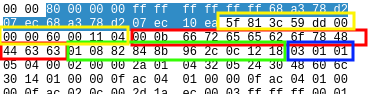
\includegraphics[width=0.8\textwidth,natwidth=610,natheight=642]{images/beacon_frame.png}
   \caption{Un exemple de beacon frame}
\end{figure}

Prenons comme exemple la figure 2.1, qui est un exemple de beacon frame obtenu avec wireshark. Les octets surlignés et ceux qui
les précédent constituent l'en-tête et ne nous intéressent pas. Les octets encadrés en jaune sont des informations ``fixes'', dans
le sens où elles sont toujours présentes dans une beacon frame. Il s'agit d'un time stamp, du beacon interval\footnote{L'intervale
de temps entre l'envoi de deux beacon frames} et quelques flags. Le reste du message illustre le fonctionnement décrit plus
haut. Ainsi, le premier octet dans le cadre rouge est 00, ce qui indique que l'information qui va suivre est le SSID\footnote{nom du
réseau wifi}. L'octet suivant est 0b\footnote{Il s'agit d'une valeur en hexadécimal valant 11 en décimal} indiquant que le SSID est
donné sur 11 octets. Les 11 octets suivants donnent le SSID au format ASCII. Le tag dans le cadre vert est 01, indiquant que 
l'information à suivre est la liste des débits supportés, et la longueur de ce champ est de 8 octets. Les 8 octets suivants indiquent
donc chacun un débit. Dernier exemple, dans le cadre bleu, le tag est 03, indiquant que l'information à venir est le canal utilisé, la 
longueur de cette information est de 01 octet et l'information est 01Ce point d'accés fonctionne donc sur le canal 1, à la
fréquence 1412\footnote{voir figure 1.1}.

Encore une fois, l'API libnl-genl nous fournit les outils pour demander au noyeau linux de faire un scan, via les commandes
NL80211\_CMD\_GET\_SCAN et NL80211\_CMD\_TRIGGER\_SCAN à envoyer dans un message netlink. Cela nous permet de récupérer toutes les
informations sur les différents réseaux contenues dans les beacon frames. Cependant, une phase de tests a montré
empiriquement que ce scan ne détectait pas toujours tous les réseaux wifi mesh. Nous avons donc pris la décision, dans le but
d'avoir les résultats les plus complets possibles, d'implémenter notre propre scanner pour exploiter nous-mêmes les beacon frames.

TCPdump est un programme généralement inclus dans les distributions linux permettant de ``sniffer'' des packets sur une interface
réseau. Ce programme se base sur libpcap\cite{SCANlib}, une librairie permettant de capturer des paquets. C'est cette librairie que
nous utiliserons. Elle permet de récupérer les messages captés par l'interface. Il est ensuite possible
d'effectuer toutes opérations souhaités sur eux.

Pour être en mesure de capter les beacon frames, il est nécessaire de régler une interface en mode monitor. De plus, puisqu'il existe
14 cannaux, il est essentiel de passer de l'un à l'autre pour tous les scanner. Ces deux opérations sont possibles avec la librairie 
libnl décrite chapitre 2, partie 1. La méthode que nous utiliserons est donc la suivante : nous paramétrons la carte réseau associée à
une interface en mode monitor sur une fréquence, puis nous utilisons les fonctions de libpcap pour écouter sur l'interface pendant 3
secondes. Pendant ce temps, à chaque réception d'une trame, nous vérifions qu'il s'agisse d'une beacon frame en analysant son champ
type. Dans ce cas, nous analysons chaque information qu'elle contient en recherchant les tags 0, 3, 113 et 114 indiquant
respectivement le SSID, le canal de fonctionnement, la configuration mesh et le MeshId. Bien sûr, seuls les beacon frames indiquant
un réseau mesh possédent les deux derniers tags. En outre, le tag 00 est toujours présent mais dans le cas d'une beacon frame 
indiquant un réseau mesh, sa longueur est de 0 bits, dû au fait qu'un réseau mesh n'est pas identifié par un SSID.

Une fois le scan répété sur chacun des 14 cannaux, nous avons donc deux listes : Une liste des réseaux ``normaux'' et une liste des
réseaux mesh. De plus, nous pouvons calculer simplement l'occcupation de chaque fréquence, et si besoin trouver la moins encombrée.
Cependant, comme évoqué précédemment, et comme le montre bien la figure 1.1, les cannaux se superposent. Il n'est pas rare, en
écoutant sur un canal, de recevoir un message envoyé sur un autre canal voisin. Ainsi, lors de la sélection de fréquence, si un canal
est déjà trés encombré, il peut être judicieux d'exclure non seulement le dit canal, mais aussi ses voisins.